
%# -*- coding:utf-8 -*-
\documentclass[UTF8]{ctexart}
\usepackage{amsmath}
\usepackage{graphicx}
\setlength{\parindent}{0em}
\begin{document}
\section{定义}
$u_n$ 收敛 $v_n$收敛,则$u_n+v_n$收敛 \\
$\sum_{n=0}^\infty \frac{1}{n^a}
\begin{cases} a>1 \mbox{收敛} \\
  0<a<1 \mbox{条件收敛} \\
  a<0 \mbox{发散} \\
  \end{cases}$

\section{反常积分审敛}
  $\sum \frac{1}{n^p}  \\
  p >1 \mbox{绝} \\
  0<p\leq1 \mbox{条} \\
  p \leq 0 \mbox{散} $ \\
  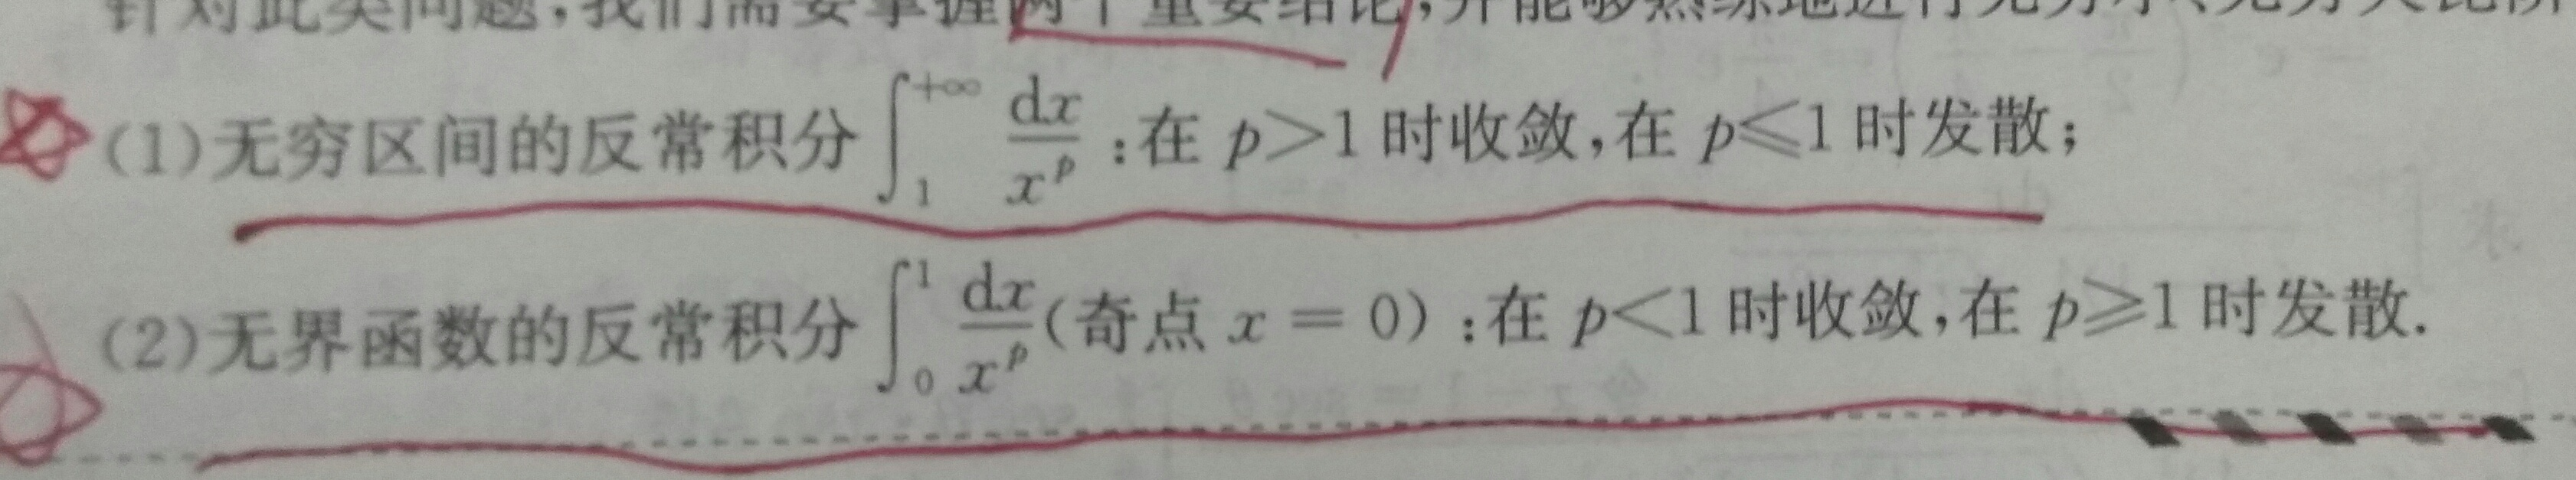
\includegraphics[width=13cm]{9345E7/2059466188.jpg}
\section{收敛区间}
缺项级数 $\lim_{n \rightarrow \infty } | \frac{u_{n+1}(x)}{u_n(x)} | $ 带上x \\
完项级数 不带x

\section{级数求和}
  $\sum_{n=1}^\infty \frac{x^n}{n} =- \ln (1-x) , x \in [-1,1)$ \\
  $\sum_{n=1}^\infty nx^{n-1} = \frac{1}{{(1-x)}^2} , x \in (-1,1)$
\section{傅里叶级数}
  $f(x) \sim S(x) = \frac{a_0}{2} + \sum_{n=1}^\infty (a_n \cos{\frac{n  \pi x}{l}
   + b_n \sin \frac{n\pi x}{l}  })$

  $\begin{cases}
  a_n=\frac{1}{l} \int_{-l}^l f(x) \cos \frac{n \pi x}{l} dx (n=0,1,2, \ldots) \\
  b_n=\frac{1}{l} \int_{-l}{l} f(x) \sin \frac{n \pi x}{l} dx (n=1,2,3,\ldots)
  \end{cases}$

\end{document}
